\documentclass[11pt]{scrartcl}
\usepackage[scale=1.5]{ccicons}
\usepackage[notextcomp]{kpfonts} 
\usepackage[margin=1.0in]{geometry}
\usepackage{amsthm,amssymb,amsmath}
\usepackage[]{graphicx}
\usepackage{subcaption}
\usepackage{enumitem}
\usepackage{bm}
\usepackage{tabu}
\usepackage{mathtools}
\usepackage{tikz}
\usepackage{tikz-3dplot}
\usepackage{xcolor}
\usepackage{colortbl}
\usepackage{wasysym}



\usepackage{color}
\definecolor{darkblue}{rgb}{0, 0, .6}
\definecolor{grey}{rgb}{.7, .7, .7}
\usepackage[breaklinks]{hyperref}
\hypersetup{
	colorlinks=true,
	linkcolor=darkblue,
	anchorcolor=darkblue,
	citecolor=darkblue,
	pagecolor=darkblue,
	urlcolor=darkblue,
	pdftitle={},
	pdfauthor={}
}
%\usepackage{fancyhdr}
%\thispagestyle{fancy}
%\lhead{Math 107}
%\chead{Lesson Plans}
%\rhead{Spring 2018}
%\lfoot{}%\scriptsize This work is licensed under the \href{http://creativecommons.org/licenses/by-sa/3.0/us/}{Creative Commons Attribution-Share Alike 3.0 License}.} 
%\cfoot{}
%%\rfoot{\ccbysa}
%\renewcommand{\headrulewidth}{.4pt}
%\renewcommand{\footrulewidth}{.4pt}

\theoremstyle{definition}
\newtheorem{theorem}{Theorem}
\newtheorem*{theorem*}{Theorem}
\newtheorem{acknowledgement}[theorem]{Acknowledgement}
\newtheorem{algorithm}[theorem]{Algorithm}
\newtheorem{axiom}[theorem]{Axiom}
\newtheorem{case}[theorem]{Case}
\newtheorem{claim}[theorem]{Claim}
\newtheorem*{claim*}{Claim}
\newtheorem{conclusion}[theorem]{Conclusion}
\newtheorem{condition}[theorem]{Condition}
\newtheorem{conjecture}[theorem]{Conjecture}
\newtheorem{corollary}[theorem]{Corollary}
\newtheorem{criterion}[theorem]{Criterion}
\newtheorem{definition}[theorem]{Definition}
\newtheorem{example}[theorem]{Example}
\newtheorem{exercise}[theorem]{Exercise}
\newtheorem{journal}[theorem]{Journal}
\newtheorem{lemma}[theorem]{Lemma}
\newtheorem{notation}[theorem]{Notation}
\newtheorem{problem}[theorem]{Problem}
\newtheorem*{problem*}{Problem}
\newtheorem{proposition}[theorem]{Proposition}
\newtheorem{remark}[theorem]{Remark}
%\newtheorem{solution}[theorem]{Solution}
\newtheorem{summary}[theorem]{Summary}
\newtheorem{skeleton}[theorem]{Skeleton Proof}
\newtheorem{activity}[theorem]{Activity}
\newtheorem{intuitivedef}[theorem]{Intuitive Definition}

\DeclareMathOperator{\spn}{span}
\DeclareMathOperator{\Char}{Characteristic}
\DeclareMathOperator{\Aut}{Aut}
\DeclareMathOperator{\stab}{Stab}
\DeclareMathOperator{\Stab}{Stab}
\DeclareMathOperator{\orb}{\mathcal{O}}
\DeclareMathOperator{\lcm}{lcm}
\DeclareMathOperator{\gl}{GL}
\DeclareMathOperator{\Ker}{Ker}
\DeclareMathOperator{\Z}{\mathbb{Z}}
\DeclareMathOperator{\C}{\mathbb{C}}
\DeclareMathOperator{\R}{\mathbb{R}}
\DeclareMathOperator{\N}{\mathbb{N}}
\DeclareMathOperator{\Q}{\mathbb{Q}}
\DeclareMathOperator{\A}{\mathbb{A}}
\DeclareMathOperator{\Gal}{Gal}
\DeclareMathOperator{\PS}{\mathcal{P}}
\DeclareMathOperator{\acc}{acc}


\newenvironment{solution}{\begin{proof}[Solution]}{\end{proof}}
\newcommand{\comment}[1]{%
  \text{\phantom{(#1)}} \tag{#1}
}


%Useful for cut and paste
%\begin{enumerate}[label=\rm{(\alph*)}]

\begin{document}
\section*{Warm-Up}
Copy the following questions into your notes and then answer the questions.
\begin{enumerate}
	\item The probability of an impossible event is?
	\item The sum of the probabilities of all the single outcome events in the sample space is equal to?
	\item If two events are disjoint then they share outcomes sometimes? always? never?
	\item The total area under the normal curve is?
	\item The $z$-score of an observation is the number of standard deviations an observation is away from the$\ldots$
	\item If an observation is larger than the mean then it's $z$-score is $\ldots$
	\item Two sets of data are normally distributed with the same mean. Data set $A$ has a standard deviation of 2.5. Data set $B$ has a standard deviation of 5. The normal curve that represents data set $A$ will be skinnier and taller? shorter and wider? than data set $B$
	\item True or False: Changing the mean of a normal curve affects the width and height of a normal curve.
	\end{enumerate}

\noindent
After the students discuss a bit, we will have the class answer clicker questions. With luck we will display these for the class and have a discussion based on agreements or disagreements.

\newpage

%\section*{Review questions}
\subsection*{Section 5.1}
Let $X$ be the outcome of rolling a 9-sided die once. Find the given probability in fraction form:
\begin{enumerate}
	\item What is the sample space?
	\item $P(X=6)$
	\item $P(X>3)$
	\item $P(X<5)$
	\item $P(X\leq 7)$
	\item $P(X \geq 4)$
	\item $P(3 \leq X \leq 7)$
	\item $P(4 \leq X \leq 9)$
	\item P(odd \textbf{OR} at most 2)
	\item P(even \textbf{AND} at most 7)
\end{enumerate}

\vspace{1cm}
\subsection*{Section 5.2}
The following table represents the results of a survey which asked people if they thought their values were threatened by Hollywood and the entertainment industry.
\begin{center}
	\begin{tabular}{lllll|l}
         & 18-29 & 30-49  & 50-69  & over 69 & Total  \\
Agree    & 1400  & 4847   & 4823   & 3910    & 14,980 \\
Disagree & 2842  & 6976   & 5661   & 4236    & 19,715 \\ \hline
Total    & 4242  & 11,823 & 10,484 & 8146    & 34,695
\end{tabular}
\end{center}
Use the table to answer the following questions:
\begin{enumerate}
	\item Find the probability that a randomly selected person agreed with the statement.
	\item Find the probability that a randomly selected person was between 30 and 49 years of age.
	\item Find the probability that a randomly selected person was 18-29 years of age \textbf{OR} over 69.
	\item Find the probability that a randomly selected person was 50-59 years of age \textbf{AND} disagreed with the statement?
	\item Find the probability that a randomly selected person was 50-59 years of age \textbf{OR} disagreed with the statement? 
\end{enumerate}


\newpage
\subsection*{Section 5.1/5.2}
Use the spinner to find the following probabilities:
\begin{center}
	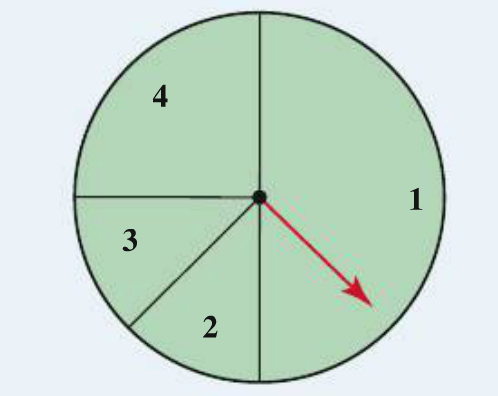
\includegraphics{Spinner}
\end{center}
\begin{enumerate}
	\item P(1)
	\item P(2)
	\item P(3)
	\item P(4)
	\item Are all outcomes equally likely?
	\item P(odd number)
	\item P(even number)
	\item P(not 2)
	\item P(at least 2)
	\item P(at most 4)
\end{enumerate}

\vspace{1cm}

\subsection*{Section 5.5}
A total of 940 healthy, pregnant women between 20 and 34 years of age participated in a study. The distribution of their pregnancies was symmetric and unimodal with a mean of 278 days and standard deviation of 8 days. Find the probabilities that a women from the study had a pregnancy that lasted:
\begin{enumerate}
	\item less than 260 days
	\item more than 289 days
	\item between 265 and 297 days
	\item A baby that is born in the 8.7th percentile is considered premature and at risk of serious health complications. After what day is a baby no longer considered premature?
\end{enumerate}

\newpage

\subsection*{Section 5.4}
\begin{problem}
	Battery lifetime is normally distributed with an average lifetime of 500 hours with a standard deviation of 61 hours. A package of batteries that Justin recently bought to use with his earphones appears to have batteries that last for 30 days. Find the z-score of the package of batteries that Justin bought. \textbf{Make sure your units match.}
\end{problem}


\begin{problem}
	A shoe manufacturer is gathering information regarding men's shoe sizes. The company found that men's shoe sizes are normally distributed with a mean size of 11 and a standard deviation of 1.5. Dylan recently went to buy shoes before starting summer classes. He bought shoes of size 9. Find the z-score for Dylan's shoe size.
\end{problem}


\begin{problem}
	 Windows Surface tablets have a mean battery life of 50 hours and a standard deviation of 12 hours. Stephanie wanted to see if her tablet fell within a ``normal range" and measure how many hours she went before having to recharge her tablet. She found that her tablet would work for 35 hours before needing to be recharged. Find the z-score for Stephanie's tablet.
\end{problem}


\begin{problem}
	Recently Nathaniel broke a string on his cello and had to replace it. When he went into the store to buy a new string the clerk told him that the lifetime of the string was normally distributed with a mean lifetime of 5 years and a standard deviation of 1.2 years. Nathaniel's last string lasted for 7.5 years. Find the z-score for that strings life.
\end{problem}

\vspace{1cm}
\subsection*{Section5.4}

\begin{problem}
	Kayla is a triathlon athlete. In the last triathlon Kayla participated in she finished the swimming portion in 53.2 minutes. After talking to the officials she found that the data was normally distributed with an average swimming time of 44 minutes and a standard deviation of 6 minutes. Find the z-score of Kayla's swimming time. 
\end{problem}


\begin{problem}
	In her nursing class Alyssia learned that the number of hours that Advil is effective for is normally distributed with a mean time of effectiveness of 4.7 hours and a standard deviation of 45 minutes. Alyssia knows from her own experience that when she takes Advil she won't have to take it again until 6 hours later. Find the z-score of the effectiveness of Advil for Alyssia. 
\end{problem}


\begin{problem}
	In Hawaii, Maggie was part of a gym. It turns out the number of minutes people spend at the gym are normally distributed with an average time of 90 minutes and a standard deviation of 20 minutes. Maggie typically stays for 75 minutes. Find the z-score of how long Maggie stays at the gym.	
\end{problem}

\begin{problem}
	A certain cooking sauce is sold in jars marked that they contain 500 grams of sauce. The jars are filled by a machine. The actual weight of the sauce is normally distributed with a mean of 505 grams of sauce with a standard deviation of 2.4 grams. What is the z-score of a jar that weighs 500 grams?	
\end{problem}

\newpage

\subsection*{Section 5.5}
\begin{problem}
	The 2014 draft picks for NBA basketball teams have heights that are approximately normally distributed with mean 79.1 inches and standard deviation 3.0 inches. The $z$-score for the tallest 2014 draft pick, Walter Tavares, is 2.63. What is Tavares's height? Round to the ones place.
\end{problem}

\begin{problem}
	The hourly temperatures at Eppley Airfield Airport in Omaha, Nebraska, in May 2014 are approximately normally distributed with a mean of 64.4$^\circ$F and standard deviation 12.2$^\circ$F. The $z$-score of the highest temperature is 2.59. What is the highest temperature?	
\end{problem}

\begin{problem}
	The lengths of songs played on Friday, April 18, 2014 on Live 105. The lengths of the songs are approximately normally distributed with mean 232.93 seconds and standard deviation 49.63 seconds. The shortest song played was ``Fell in Love with a Girl" by the White Stripes. The song's length has a $z$-score of -2.48. What is the length of the song?
\end{problem}

\begin{problem}
	The age distribution of inmates on death row in Alabama is approximately normal with mean 43.0 years and standard deviation 9.7 years. The $z$-score of the youngest inmate is -2.16. What is his age?
\end{problem}

\vspace{1cm}

\subsection*{Section 5.5}
A professor gives a test to a trigonometry class. The scores are approximately normally distributed with mean 78 points and standard deviation 7 points.
\begin{enumerate}
	\item The professor usually uses 90 points as the cutoff for an A. If the professor uses this cutoff, what percentage of the students would get As?
	\item The professor usually uses 75 to 89 points as the cutoff for a B. If the professor uses this cutoff, what percentage of the students would get Bs?
	\item The professor usually uses 0 to 45 for an F. If the professor uses this cutoff, what percentage of the students would get Fs?
	\item If the professor decides to give As to approximately 8\% of the students but not less than 8\%, what should the cutoff score for an A be?
	\item The professor also decides to gives Fs to approximately 6\% of the students but not less than 6\%, what should the cutoff score for an F be?
	\item The professor decides to give Bs to students who score above the 65th to 92nd percentiles. What should the cutoff for B be?
\end{enumerate}

\newpage

\subsection*{Section 5.5}
Scores on the Wechsler IQ test are normally distributed with mean 100 points and standard deviation 15 points.
\begin{enumerate}
	\item A student's IQ is at the 95th percentile. Find the student's IQ score.
	\item Mensa is a high-IQ society. Membership is open to people who have attained a score within the upper 2 percent of the general population on an approved intelligence test. What is the cutoff score on the Wechsler IQ test in order to qualify for Mensa?
	\item A person scores 130 points on the Wechsler IQ test. Is this an unusual score? Why or why not?
	\item Alexis Martin, who just turned 3 years old, has an IQ of 160 points. What is her $z$-score? Does she have an unusual IQ?
	\item A student's IQ is at the 42nd percentile. Find the student's IQ score.
	\item A student's IQ is at the 54th percentile. Find the student's IQ score.
	\item A student's IQ is at the 12th percentile. Find the student's IQ score.
\end{enumerate}



\end{document}
